\section{Durchführung}
\label{sec:Durchführung}

Die Schaltung zur Durchführung dieses Versuches ist in der \autoref{fig:schaltung} zu sehen. Die Franck-Hertz-Apparatur 
wird in dem Abschnitt \ref{sec:Theorie} näher beschrieben. Die Glühkathode wird mit einer konstanten Gleichspannung betrieben. 
Die Beschleunigungsspannung $U_{\text{B}}$ und die Auffängerspannung $U_{\text{A}}$ sind variabel und können an den XY-Schreiber 
angeschlossen werden. Die Temperatur wird mit einem Temperaturregler gesteuert und an einem digitalen Thermometer abgelesen. 
Der Auffängerstrom wird mit einem Picoamperemeter gemessen und auf die Y-Achse des XY-Schreibers gelegt. 

\begin{figure}[H]
    \centering
    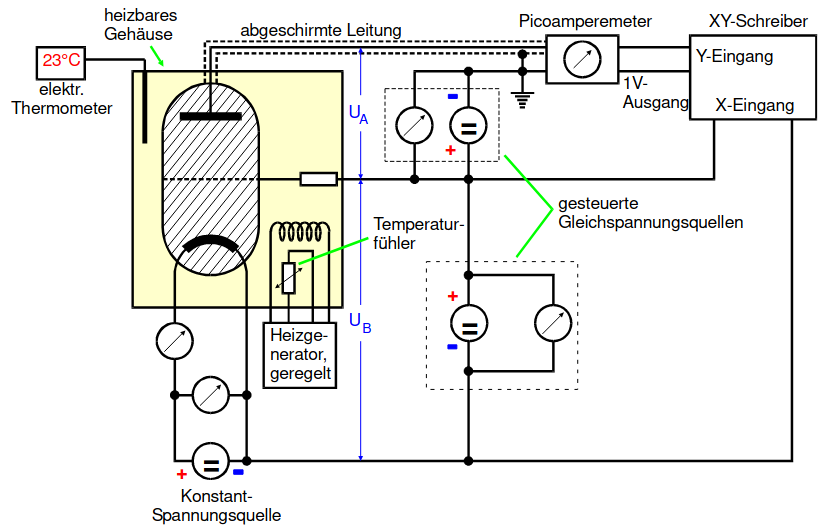
\includegraphics[width=\textwidth]{bilder/schaltung.png}
    \caption{Die Schaltung zur Aufnahme einer Franck-Hertz-Kurve \cite{anleitung}.}
    \label{fig:schaltung}
\end{figure}

\noindent Der XY-Schreiber kann ein Blatt elektrostatisch festigen und auch den Stift absetzen oder schweben lassen. Auf die X-Achse wird
eine Spannung gelegt, es ist darauf zu achten, dass der zu betrachtete Spannungsbereich möglichst das gesamte Blatt einnimmt. 
Die Skalierung sowie der Nullpunkt kann mithilfe von Rädchen eingestellt werden. Nach erfolgreicher Messung ist es für eine vernünftige
Auswertung wichtig, dass die X-Achse einmal skaliert wird, also das auf dem Papier mehrere Punkte markiert werden.

\subsection{Messung der integralen Energieverteilung}

    Für die Aufnahme der integralen Energieverteilung der Elektronen wird der Auffängerstrom in Abhängigkeit der Bremsspannung aufgetragen. 
    Die Beschleunigungsspannung ist konstant und wird auf $U_{\text{B}} = \SI{11}{\volt}$ eingestellt. Die Bremsspannung durchläuft ihren 
    kompletten Wertebereich von $\SI{0}{\volt} - \SI{10}{\volt}$. Die Messung wird einmal bei Raumtemperatur und einmal bei etwa $T = \SI{140}{\celsius} - \SI{160}{\celsius}$
    durchgeführt. 

\subsection{Messung der Franck-Hertz-Kurve}

    Bei der Aufnahme einer Franck-Hertz-Kurve wird die Beschleunigungsspannung von $U_{\text{B}} = \SI{0}{\volt}- \SI{60}{\volt}$ variiert und auf die 
    X-Achse gelegt. Die Bremsspannung ist konstant auf etwa $U_{\text{A}} = \SI{1}{\volt}$ eingestellt. Auf der Y-Achse liegt wieder der Auffängerstrom. 
    Die Messung wird für zwei Temperaturen im Bereich von $T = \SI{160}{\celsius} - \SI{190}{\celsius}$ durchgeführt. 

\noindent Der Aufbau des Expermentes vor Ort ist in der \autoref{fig:foto_aufbau} zu sehen. Links befindet sich der Temperaturregler unterhalb der Gleichspannungsquelle
für die Glühkathode. Im Vordergrund ist der XY-Schreiber zu sehen, im Hintergrund die Franck-Hertz-Apparatur. Rechts steht das digitale Thermometer auf dem Amperemeter, 
welches auf der variablen Spannungsquelle für die Beschleunigungsspannung und die Bremsspannung steht. 

\begin{figure}[H]
    \centering
    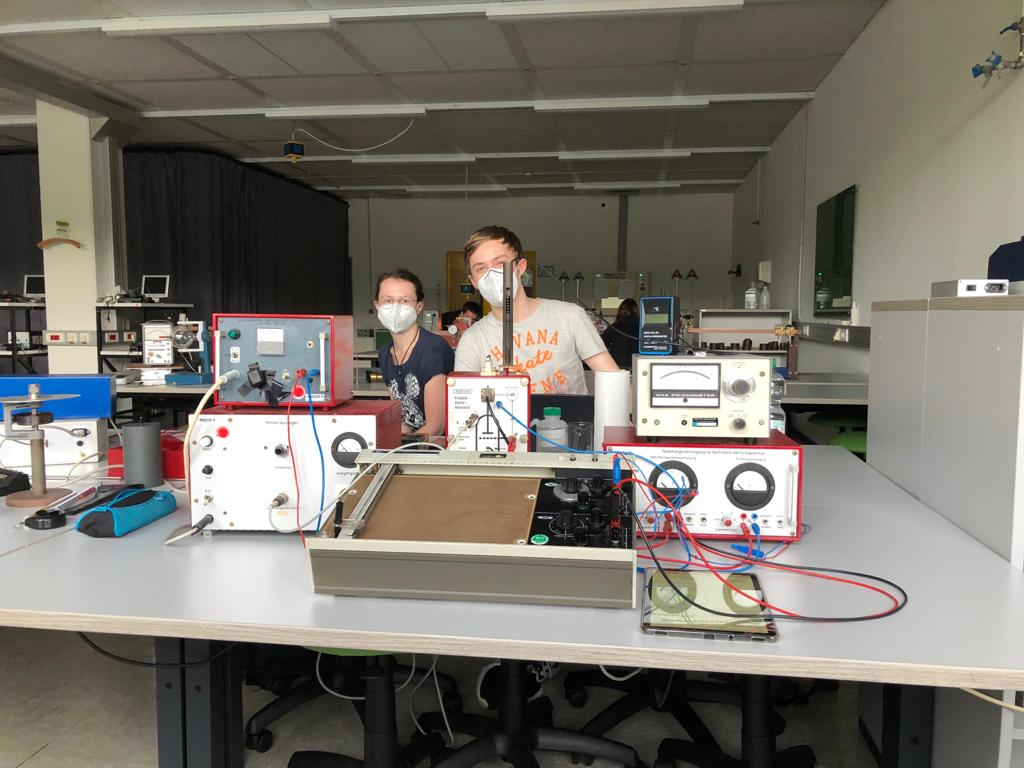
\includegraphics[width=0.6\textwidth]{bilder/foto_aufbau.jpeg}
    \caption{Der Aufbau des Experimentes vor Ort.}
    \label{fig:foto_aufbau}
\end{figure}